
\section{Other applications of the method}
\label{chapfin}
In this chapter, I present ongoing work and preliminary observations about other topics, studied with the method preseted previously.

\subsection{Elastohydrodynamic lift near a soft wall}

\begin{figure}[H]
	\centering
	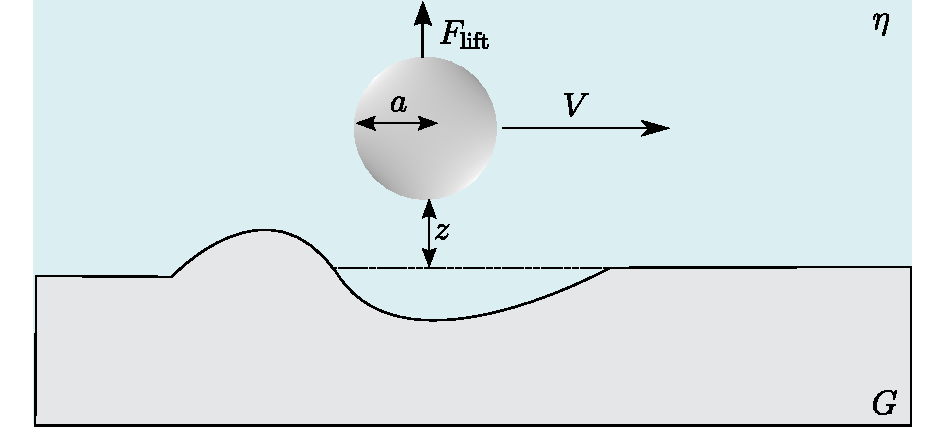
\includegraphics{02_body/chapter4/images/EHD_forces/drawing_system.pdf}
	\caption{Schematic of a spherical colloid of radius $a$  immersed in a fluid of viscosity $\eta$ sliding at a velocity $V$ above an incompressible and linear-elastic substrate of shear elastic modulus $G$. From the elastohydrodynamic interaction between the particle and the soft wall arises a net lift force $F_\mathrm{lift}$ (see Eq.~(\ref{Eq.lift_deter})).}
	\label{fig.shema_EHD}
\end{figure}



Elastohydrodynamics (\gls{EHD}) is the field of mechanics that couples elasticity and hydrodynamics. We here focus particularly on \gls{EHD} in the context of lubrication, which describes the relative motion of immersed objects in a near-contact regime. Lubrication \gls{EHD} is present at many length and time scale. Examples of relevant phenomena and systems include, kilometrics landslides \cite{campbell_self-lubrication_1989}, roller bearings \cite{hamrock_fundamentals_2004} and blood-cell motion in microfluidic devices \cite{byun_characterizing_2013, higgins_sickle_2007, cohen_hydrodynamics_2013}. Recently, the problem of a free particle that can sediment, slide or roll near a soft surface has been treated  \cite{sekimoto_mechanism_1993,skotheim_soft_2004,skotheim_soft_2005,beaucourt_optimal_2004,salez_elastohydrodynamics_2015,bertin_soft-lubrication_2021}. As the particle slides near the surface, the hydrodynic stresses deform the soft wall surface. This deformation induces a symmetry breaking of the contact geometry. Hence, a net normal force emerges and is applied to the objects. Furthermore, if a particle is sliding due to its own weight, this lift force can be self-sustained. The first experimental quantitative observation of the lift effect has been done at the macroscopic scale using negatively-buoyant centimetric cylinders immersed in a viscous fluid, that were sliding down a tilted wall coated with an elastic layer. The authors show that the self-sustained \gls{EHD} lift reduces the coefficient of dynamic friction by nearly an order of magnitude and suggest that this \gls{EHD} force could partially explain phenomena such as reduced wear in animal joints and long-runout landslides. The \gls{EHD} lift force has also recently been measured at the microscopic-scale, using micron-sized colloidal spheres in micro-channels under flow. However, in all these experiments,  the motion is deterministic and induced by an external force or flow. In the context of my thesis, we further wonder wether spontaneous Brownian motion, and thus thermal fluctuations could trigger such an effect in some temporal range. In the lubrication ``\gls{EHD}" theory, considering a sphere of radius $a$ moving at constant velocity $V$, in a solvent of viscosity $\eta$, and at a distance $z$ from a thick (with respect to the particle radius), incompressible, linear-elastic substrate of shears elastic modulus $G$, the lift force $F_\mathrm{lift}$ reads \cite{skotheim_soft_2004}:

\begin{equation}
	F_\mathrm{lift} \sim 0.41\frac{\eta^2 V^2}{G} \frac{a^{5/2}}{z^{5/2}} ~,
	\label{Eq.lift_deter}
\end{equation}

 where the $0.41$ factor has been computed by Bertin \textit{et al.} \cite{bertin_soft-lubrication_2021}. To incorporate fluctuations into this deterministic picture, a simple idea is to replace the velocity $V$ in Eq.~(\ref{Eq.lift_deter}) by the typical horizontal thermal velocity $\sqrt{k_\mathrm{B}T / m}$ obtained through the Maxwell-Boltzmann distribution , leading the following estimate of an hypothetical Brownian \gls{EHD} lift force:

\begin{equation}
	F_\mathrm{lift, Brown} \sim 0.41\frac{\eta ^2 k_\mathrm{B}T}{G\rho_\mathrm{p} a^{1/2} z^{5/2}} ~.
	\label{Eq.lift_brown}
\end{equation}


From this equation, we can observe a counterintuitive effect: as the particle radius (and thus the surface of contact) decreases, the the \gls{EHD} force $F_\mathrm{lift, Brown}$ increases. Taking typical biophysical values such as $G \simeq 10$ kPa, $\rho_\mathrm{p} = 1350$ kg.m$^{-3}$ (proteins density) and $a=100$ nm, we see that the Brownian \gls{EHD} force is in the piconewton range. The latter range is comparable to other surface forces, which means that microscopic entities in biology and nanoscience may spontaneously trigger Brownian \gls{EHD} couplings, notably their dynamics. However, it is important to note that it is only a simple estimate and which contains a high risk of conceptual failure associated, for example, to the lake of compensating drift at equilibrium. 

\subsubsection{PolyDimethylSiloxane}
To do the soft coating experimentally, we use PolyDimethylSiloxane (\gls{PDMS}) which is widly use for fabrication in microfluidics and also in shampoo \cite{im_shampoo_2012} or food\footnote{ \gls{PDMS} is used as an antifoaming agent in food and is identified by the European food additive number E900.}. \gls{PDMS} is a silicone-based organic polymer wwhich chemical formula is:

\begin{equation}
	\mathrm{CH_3[Si(CH_3)_2 O]}_n \mathrm{Si(CH3)_3} ~,
\end{equation}

where $n$ is the number of $\mathrm{Si(CH_3)_2 O}$ dimethyl groups. By mixing a solution of \gls{PDMS} chains with a curring agent containing hydrosilane groups ($\mathrm{SiH}$), bonds or crosslink between different \gls{PDMS} chains are appearing, as shown in Fig.~\ref{fig.crosslink}.




\begin{figure}[H]
	\centering
	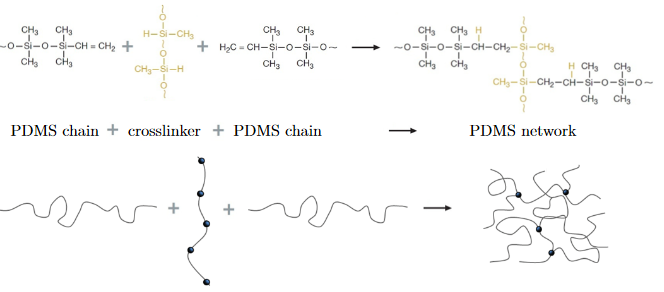
\includegraphics[scale = 0.8]{02_body/chapter4/images/EHD_forces/figure_cross.png}
	\caption{Figure taken from \cite{tucher_analysis_2016}. Examples of crosslinking reaction between the \gls{PDMS} chains and a curing agent containing hydrosilane groups.}
	\label{fig.crosslink}
\end{figure}


Due to the crosslinker, the \gls{PDMS} turns into an elastomer, modelled as an incomprehensible and linear-elastic solid. Some of its characteristics are to be hydrophobic and to exhibit strong gas permeability \cite{xia_soft_1998}. The elastic modulus $G$ of the crosslinked \gls{PDMS} can be tuned by changing the mixing ratio of base polymer solutions and curing agent. For example, for one of the most used \gls{PDMS}, which is Sylgard 184, a mixing ratio of $10:1$ leads to an elastic modulus $G=1.5$ MPa,a $35:1$ leads to $G\simeq 100$ kPa \cite{wang_crosslinking_2014}. To prepare experimental samples, it possible to spin coat the microscope slides with the base-agent mixture before it is cured in order to have a thick soft surface coating onto the slides. However, for simplicity, we first decided to use already prepared samples sold by Ibidi, these came as soft coated Petri dishes with a coverslip on the bottom that we can directly fit into our microscope.


\subsubsection{Measuring non-conservative forces}

To measure the non-conservative forces felt by a Brownian particle diffusing on top of a soft surface, we do the exact same experiment and data analysis as the one developed in section \ref{section:expresults}. As the \gls{EHD} force does not derive from a potential, we need to extract the non-conservative forces $F_\mathrm{NC}$, to do so, by combining Eqs.~(\ref{Eq.conservative_force})~and~(\ref{Eq:Force}), the non-conservative force reads:

\begin{equation}
	F_\mathrm{NC} = F_z(z) - F_z ^\mathrm{eq}(z) ~.
\end{equation}

In Fig.~\ref{fig.ncforce} are shown the measured $F_\mathrm{NC}$ as a function of particle-wall distance, for two different elastic moduli $G=15$ and $28$ kPa. These first experiments suggest that Brownian motion might indeed trigger some non-conservative \gls{EHD} forces. This preliminary experiment will be completed in near future with additional and systematic experiments.

Specifically, we will vary three parameters, $\eta$, $G$ and $a$ to check if we can obtain a universal plot,\textit{i.e.} where $F_\mathrm{lift, Brown}$ varies linearly with $\frac{\eta^2}{Ga^{1/2}} $, as shown in Fig.~\ref{fig.ncforcenormalized} with the first experiments.

\begin{figure}[H]
	\centering
	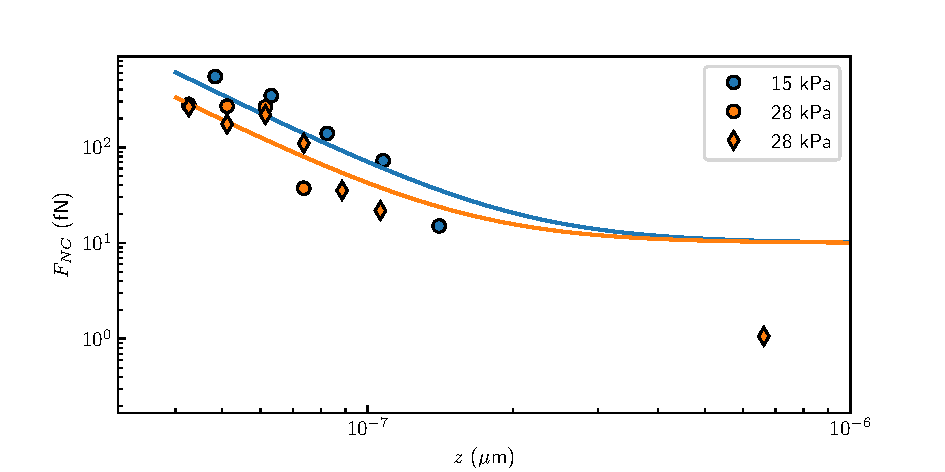
\includegraphics{02_body/chapter4/images/EHD_forces/EHD_force.pdf}
	\caption{Non-conservative forces measured experimentally as a function of particle-wall distance, for colloidal particles of radius $a=1.5 ~\mathrm{\mu m}$ diffusing in water above an incompressible and linear-elastic substrate of shear elastic moduli $G=15$ and $28$ kPa. Plain lines correspond to the Brownian \gls{EHD} prediction $F_\mathrm{lift, Brown}$ (see Eq.~(\ref{Eq.lift_brown})).~\href{https://github.com/eXpensia/Confined-Brownian-Motion/blob/main/02_body/chapter4/images/EHD_forces/global_EHD_plot.ipynb}{\faGithub}}
	\label{fig.ncforce}
\end{figure}

\begin{figure}[H]
	\centering
	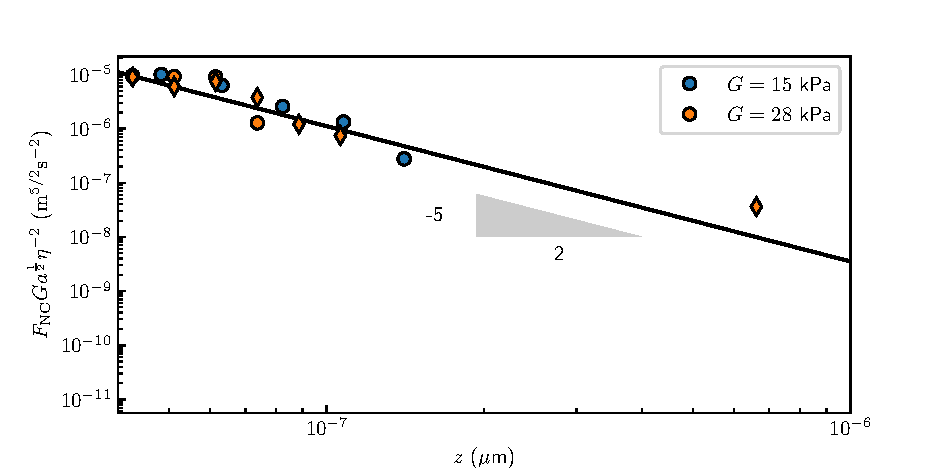
\includegraphics{02_body/chapter4/images/EHD_forces/EHD_force_rescale.pdf}
	\caption{Non-conservative forces  normalized by $ Ga^{1/2}z\eta ^{-2}$ by measured experimentally for colloidal particles of radius $a=1.5 ~\mathrm{\mu m}$ diffusing in water above an incompressible and linear-elastic substrate of shear elastic moduli $G=15$ and $28$ kPa. The plain line corresponds to the Brownian \gls{EHD} lift force $F_\mathrm{lift, Brown}$ (see Eq.~(\ref{Eq.lift_brown})).~\href{https://github.com/eXpensia/Confined-Brownian-Motion/blob/main/02_body/chapter4/images/EHD_forces/global_EHD_plot.ipynb}{\faGithub}}
	\label{fig.ncforcenormalized}
\end{figure}


\subsection{Close wall stuck motion}

\begin{figure}[H]
	\centering
	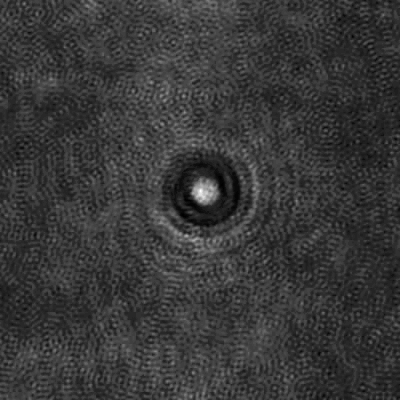
\includegraphics[scale=0.5]{02_body/chapter4/images/stucked_particle/ghost.png}
	\caption{Median of the a movie of the hologram of a stuck yet moving particle. The median is calculated over $120$ images taken every $30$ s.}
	\label{fig.ghost_stucked}
\end{figure}

When performing the experiments near a rigid wall in order to  measure the Debye length $\ell _\mathrm{D}$ (see section~\ref{sec:Eqdistrib}) as a function of the concentration of NaCl, we observed that some particles were stuck on the surface. As we first expected for this stuck particles, we did not observe any motion of the particle. However, surprisingly, in some cases we observed that some particles were slightly diffusing. This slight diffusion can be observed directly from the raw data, by looking at the median of the images of the video capture from an hologram of a stuck yet moving particle. The latter median is shown in Fig.~\ref{fig.ghost_stucked}, where we observe a blurry hologram due to the particle motion. Moreover, as we cannot properly have the background in this experiment since the particle does not diffuse enough, the statistical error is increased. The measured trajectory is shown in Fig.\ref{fig.trajectory_stuck}, where we observe that a mechanical drift happened during the experiment. This could be due to a shifting in time of the sample or the objective position, for example. The corresponding drift velocity is on the order of $2 ~ \mathrm{\mu m.h^{-1}}$ along the $x$- and $y$-axes and  $6 ~ \mathrm{\mu m.h^{-1}}$ along the $z$-axis. In the following, we look at the short-time dynamics ($t < 1$~s), since the drift over such a time scale is of the order only nanometric in position.

\begin{figure}[H]
	\centering
	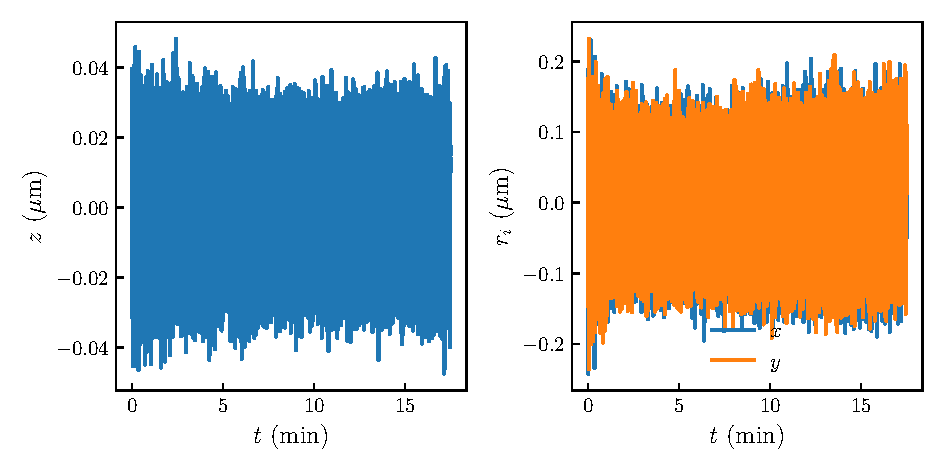
\includegraphics{02_body/chapter4/images/stucked_particle/trajectory_stucked.pdf}
	\caption{Raw trajectories measured using the Mie tracking technique for the $x$-, $y$- and $z$- axes, for a particle of radius $a=1.5 ~\mathrm{\mu m}$. The time between each frame is $\tau = 1/200$ s. ~\href{https://github.com/eXpensia/Confined-Brownian-Motion/blob/main/02_body/chapter4/images/stucked_particle/Full\%20analysis\%20trajectory_using_Dyacine_adding_x_y_distrib.ipynb}{\faGithub}}
	\label{fig.trajectory_stuck}
\end{figure}



Let us focus on the \gls{MSD}s along the $x$-, $y$- and $z$-axes are shown in Fig.~\ref{fig.MSD_stucked}. We observe that the \gls{MSD} along the $z$- axis is a constant, with $(\langle r_z^2 \rangle_t)^{1/2} = 10 $~ nm which is of the order of the tracking uncertainty (see section~\ref{chap:LM_fit}); hence, I will not physically comment the results obtained along the $z$-axis. However, on the $x$-axis, interestingly, indicating that the particle is diffusing in a potential. In addition, the collapse with the corresponding data on the y-axis suggests that the potential is isotropic along the $x$- and $y$-axis, as if the particle was adhering to the surface with some rotational diffusion. The regime, at short time is linear with $\Delta t$ showing a normal diffusion with  average diffusion coefficients (see Eq.~(\ref{averagediff}))  $\langle{D_\parallel}\rangle= \langle D_x\rangle=\langle D_y \rangle =0.14\,D_0$. This latter value is lower thanhe minimum value of $D_\parallel$, See Eq.~(\ref{Eq:etax}), which demonstrates that the associated motion is not a simple translational diffusive motion in the xy-plan.



\begin{figure}[H]
	\centering
	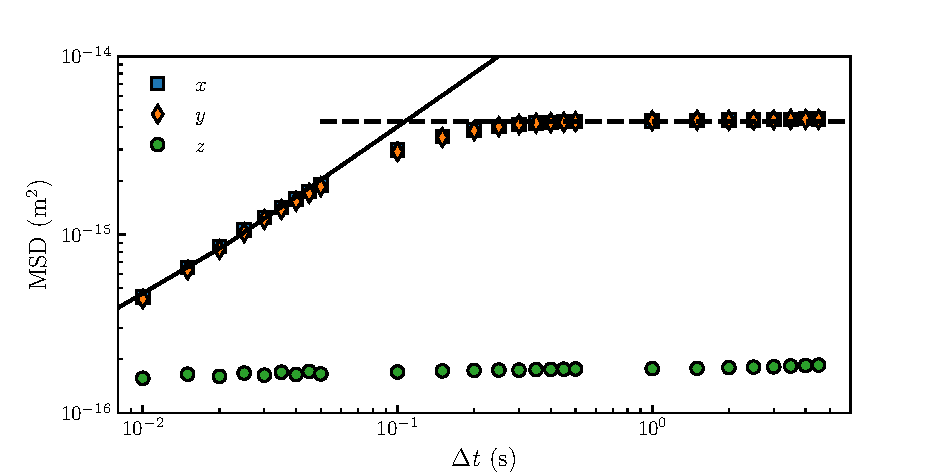
\includegraphics{02_body/chapter4/images/stucked_particle/MSD_stucked.pdf}
	\caption{Measured mean-squared displacements (MSD, see Eq.~(\ref{MSDdef})) of a particle stuck on the surface  as functions of the time increment $\Delta t$, for the three spatial directions, $x$, $y$, and $z$. The solid line is the best fit to Eq.~(\ref{averagediff}), having $\langle D_i \rangle$ as a free parameter,
		providing the average diffusion coefficient $\langle{D_\parallel}\rangle= \langle D_x\rangle=\langle D_y \rangle =0.14\,D_0$. The dashed black line is the average value of the plateau of the MSD along the $x$- and $y$-axes, \textit{i.e.} $ 4.3 \times 10 ^{-15} ~ \mathrm{m^2}$.~\href{https://github.com/eXpensia/Confined-Brownian-Motion/blob/main/02_body/chapter4/images/stucked_particle/Full\%20analysis\%20trajectory_using_Dyacine_adding_x_y_distrib.ipynb}{\faGithub}}
	\label{fig.MSD_stucked}
\end{figure}

The plateau of the MSD along  $x$ and $y$ has an average value   $4.3 \times 10 ^{-15} ~ \mathrm{m^2}$. By supposing that the particle is in a harmonic potential, we can make an estimate of the spring constant $k_\mathrm{H}$, using the relation:

\begin{equation}
	k_\mathrm{H} = \frac{  k_\mathrm{B} T}{ \lim\limits_{\Delta t \rightarrow \infty }\langle \Delta x ^2 \rangle} = \frac{8 \times 10^{-21}}{4.3 \times 10 ^{-15}} \simeq 1 ~ \mathrm{\mu N . m^{-1}}~.
\end{equation}

Beyond further understanding the origin of such a stiffness, and possibly relating it to adhesion, it would be interesting to reproduce the same study using a soft surface and see if we can observe a change of $k_\mathrm{H}$ with the elastic modulus $G$. If the latter is true, this experiment could lead to a local determination of elastic moduli using Brownian colloids attached on soft surfaces. Additionally, we can look at the displacement \gls{PDF}s $P_i$ as shown in the Fig.~\ref{fig.P_dxz_stucked}. Contrary to the result we had for a freely diffusing particle (see Fig.~\ref{fig.displacement}) we do not observe a clear non-Gaussianity here.


\begin{figure}[H]
	\centering
	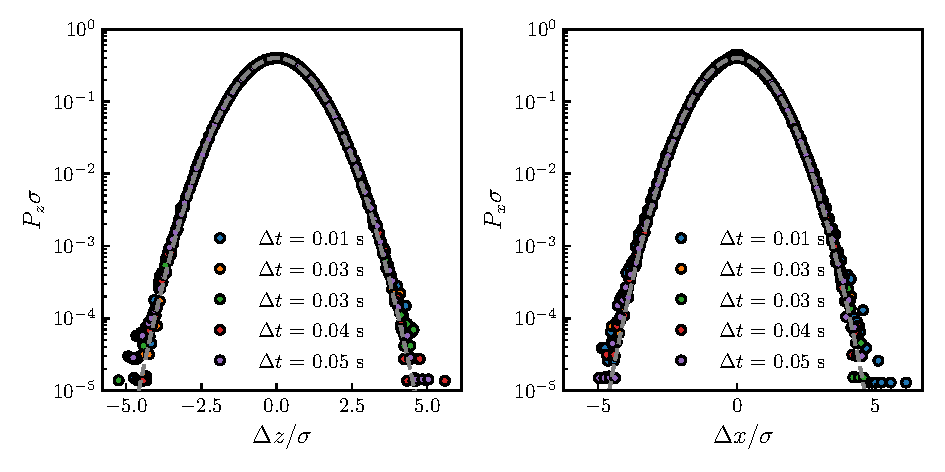
\includegraphics{02_body/chapter4/images/stucked_particle/P_xz_stucked.pdf}
	\caption{ Normalized probability density functions $P_i\,\sigma$ of the normalized displacements $\Delta x/\sigma$ and $\Delta z/\sigma$, at short times, with $\sigma^2$ the corresponding MSD (see Fig.~\ref{fig.MSD_stucked}), for different time increments $\Delta t$ ranging from 0.01~s to 0.05~s, as indicated with different colors. The gray dashed lines are normalized Gaussian distributions, with zero means and unit variances.}
	\label{fig.P_dxz_stucked}
\end{figure}


\subsection{Long-time 4th cumulent}

In this subsection we consider a cumulent of higher order than 2 (\gls{MSD}). The 4th order cumulent readss:

\begin{equation}
	C_4 (\Delta t) = \frac{1}{4!} \left(
	\left\langle [ x_i(t + \Delta t) - x_i(t) ]^4 \right\rangle_t
	- 3\left\langle [ x_i(t + \Delta t) - x_i(t) ]^2 \right\rangle_t ^2
	\right) ~.
	\label{c4}
\end{equation}

For a Gaussian-distributed variable $x$ , $C_4$ is given by the second order moment as $ \langle \Delta x^4 \rangle_t  = \langle \Delta x ^2 \rangle _t ^2 $. Therefore, the literature often overlooks higher moments as they rarely give additional information. However, as it has been shown along this manuscript, confined Brownian motion exhibits non-Gaussian statistical properties, as shown in Fig.~\ref{fig.displacement}. Thus, it becomes interesting to study higher-order cumulents. We work on this project with David Dean, Thomas Guérin and Arthur Alexandre who are experts in stochastic theory. They found an interesting behavior for the 4th cumulent in parallel displacement to the wall, for which the Langevin equation along the $x$-axis is given by:

\begin{equation}
	\mathrm{d}x = \sqrt{2D_\parallel(z)} \mathrm{d}B_t
	\label{c4.dx}
\end{equation}

In this context, Eq.~(\ref{c4}) can be simplified in two regimes [unpublished work by Alexandre \textit{et al.}], for $\Delta t \ll 1 $, one has:

\begin{equation}
	\lim\limits_{\Delta t \rightarrow 0 } C_4 (\Delta t) = \frac{\Delta t ^2}{2}
	\left(
	\langle D_\parallel ^2 \rangle - \langle D _\parallel \rangle ^2 
	\right)~,
\end{equation}

where the averages are done over the equilibrium distribution $P_\mathrm{eq}$. The forth-cumulent thus varies as $\Delta t ^2$ at short time. In the limit $\Delta t \rightarrow \infty$, Eq.~(\ref{c4}) can be simplified to:

\begin{equation}
	\lim\limits_{\Delta t \rightarrow \infty } C_4 (\Delta t) = C_4 ^0 \Delta t - C^1 _4 ~,
\end{equation}

where $ C_4 ^0$ and $ C_4 ^1$ are constants that depend on the equilibrium distribution $P_\mathrm{eq}$, and can be written as functions of $B$, $\ell _ \mathrm{D}$ and $\ell _\mathrm{B}$. Unlike the first and second moments of the parallel displacement (the average displacement $\langle Delta x \rangle_t$ and the \gls{MSD} $\langle \Delta x ^2 \rangle_t $ respectively), the 4th cumulent exhibits a peculiar regime at late times. This result is thus interesting as it gives a new statistical observable to characterize the long-term trajectory. If this prediction is verified, it could be added to our inference method (see section \ref{section:expresults}) in order to gain precision and robustness.

As we are only interested in the $x$- and $y$-axis displacements to show this result, we do not need 3D tracking. Thus, we only need to find the hologram centroids, and therefore we can use faster algorithms than the one employed in the full the Mie framework. To do so, we use the Trackpy package \href{https://github.com/soft-matter/trackpy}{\faGithub} \cite{allan_soft-mattertrackpy_2021} which implements the Crocker–Grier algorithm \cite{crocker_methods_1996}. The latter permits tracking the centroids of hundreds of colloids rapidly. Trajectories recorded this way are shown in Fig.~\ref{fig.trajtrackpy}.
\begin{figure}[H]
	\centering
	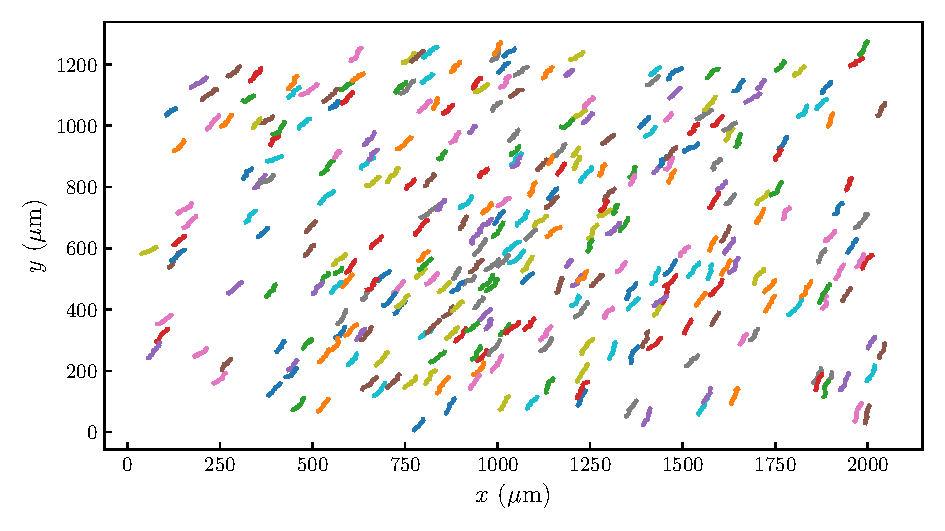
\includegraphics{02_body/chapter4/images/4th_cumulent/trajectories.pdf}
	\caption{Trajectories of 300 particles of commercial radius $a=2.5 ~ \mathrm{\mu m}$. The trajectories are composed of 10000 points with each, with time step $\tau = 0.05$~s. }
	\label{fig.trajtrackpy}
\end{figure}
From the data, we can compute the 4th cumulent using Eq.~(\ref{c4}) and we do observe a linear regime as shown in Fig.~\ref{fig.forth}. However, this experiment has only been done once so far: it is thus a preliminary result that needs further confirmation.
\begin{figure}[H]
	\centering
	
\includegraphics{02_body/chapter4/images/4th_cumulent/fourth.pdf}
	\caption{Experimentally measured 4th cumulent of the transverse displacement as a function of time increment. The plain line corresponds to a linear relation, as in Eq.~(\ref{c4.dx})}
	\label{fig.forth}
\end{figure}
\subsection{Sample ageing}

While doing the experiments on the soft surfaces, we observed that the images were becoming blurry with time. An example is shown in Fig.~\ref{fig.3hours1p5kpa} where we can see microscope images separated by three hours.


\begin{figure}[h]
	\centering
	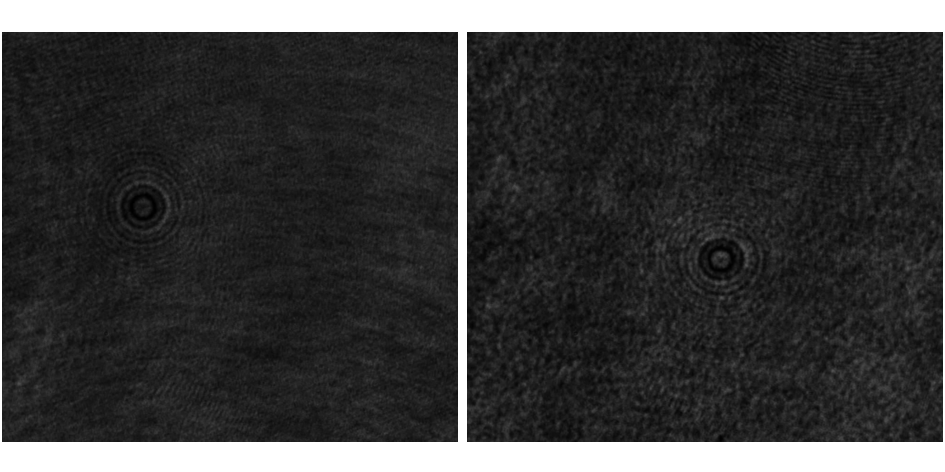
\includegraphics{02_body/chapter4/images/ageing/diffusing_particle_1p5kpa_3hours.pdf}
	\caption{Hologram of a particle diffusing above a soft surface ($G=1.5$~kPa). The image on the right has been taken 3 hours after the one on the left. The images are $45~\mathrm{\mu m}$ wide and $50~\mathrm{\mu m}$ tall. }
	\label{fig.3hours1p5kpa}
\end{figure}

Trying to find the origin of this effect, we focused on the interface between the soft PDMS layer and the glass substrate. Doing so, we observed a structure that looks like bubbles, as shown in Fig.\ref{fig.bubbles}. We observe that this effect happens faster as the PDMS is softer (lower modulus) and the bubbles seem to be also bigger. One of the ideas we have to explain this phenomenon comes from the high gas permeability of PDMS that could lead to a gas accumulation between the PDMS and the glass. The origin of this gas would come from the naturally present gas molecules inside the colloid suspension. Other possible scenarios include swelling and osmocapillarity in the PDMS. This observation will be the subject of future work. 


\begin{figure}[h]
	\centering
	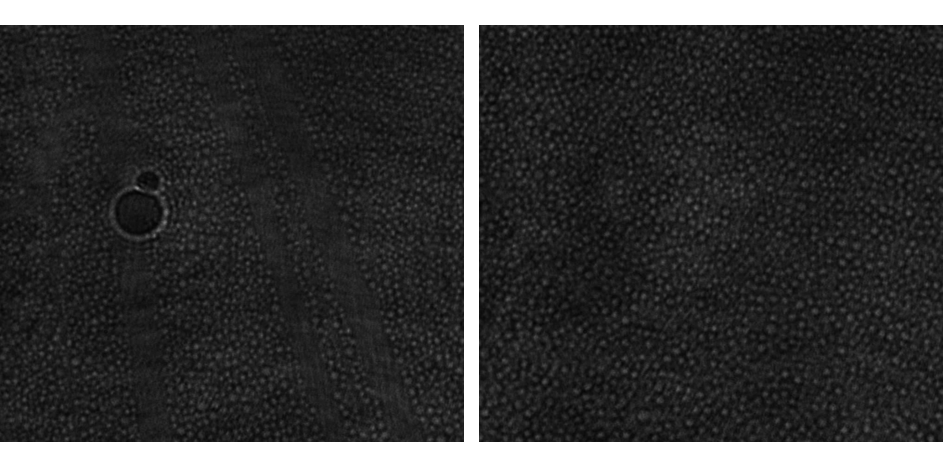
\includegraphics{02_body/chapter4/images/ageing/bullbles_1p5kpa_3hours.pdf}
	\caption{Images of the glass-PDMS ($G=1.5$~kPa) interface, three hours after water has been introduced atop the sample. The images are $45~\mathrm{\mu m}$ wide and $50~\mathrm{\mu m}$ tall.}
	\label{fig.bubbles}
\end{figure}
